\documentclass[12pt]{article}

\usepackage{amsmath}
\usepackage{hyperref}
\usepackage{graphicx}
\usepackage{float}
\usepackage{caption}

\setlength{\parskip}{1em}

\begin{document}

\begin{titlepage}
\centering
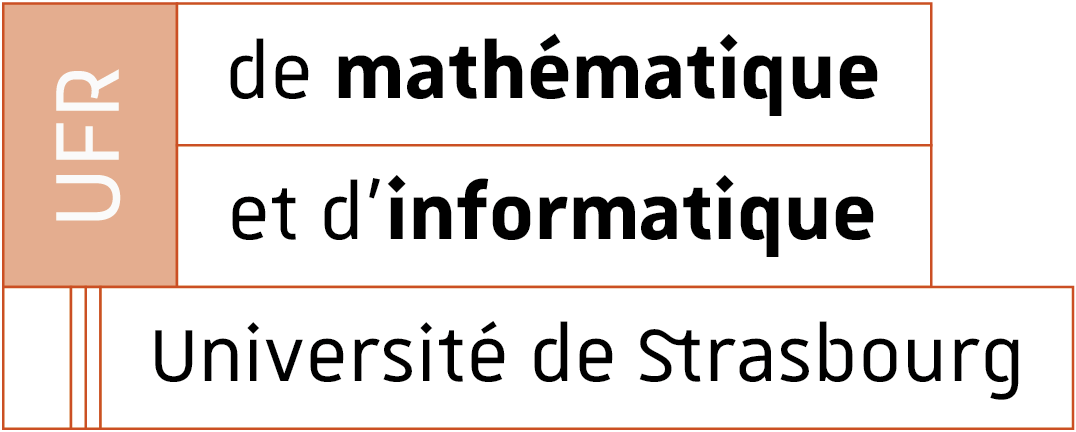
\includegraphics[width=0.5\textwidth]{images/logo_ufr.png}\par\vspace{1cm}
\vspace{1.5cm}
{\huge\bfseries ExaMA WP1 - Vegetation\par}
\vspace{2cm}
{\Large Giulio Carpi Lapi, Pierre-Antoine Senger\par}
\vfill
supervised by\par
Pierre Alliez and Vincent Chabannes

\vfill

% Bottom of the page
{\large Date: \today\par}
\end{titlepage}

\tableofcontents
\newpage

\section{Abstract}
(add sources)
Urban areas are complex ecosystems influenced by various factors, among which 
vegetation, especially trees, holds significant importance. Trees play a crucial 
role in shaping microclimates, reducing energy consumption, and enhancing overall 
livability. This project aims to integrate vegetation, specifically trees, into 3D 
geometric models of urban environments to improve the accuracy and realism of thermal 
and energy simulations. Utilizing data from open sources like OpenStreetMap , the project 
seeks to identify tree positions and attributes within urban landscapes and develop 
a library of 3D tree models for integration into terrain meshes. The project follows
 a roadmap with defined milestones to deliver versions V0, V1, and V2 by specified 
 deadlines. Through this effort, the project aims to provide valuable insights for
  urban planners, architects, and policymakers, ultimately contributing to the
   creation of more sustainable and resilient cities.

\subsection{Main Objectives}
The primary objective of this project is to integrate vegetation, particularly 
trees, into 3D urban models to enhance the accuracy of thermal and energy simulations. 
Additionally, specific objectives include:
\begin{itemize}
    \item Extracting tree data from OpenStreetMap
    \item Generating 3D tree models
    \item Integrating tree models into terrain meshes
    \item Simulating shading effects on buildings (Feel++ ray tracing)
    \item Simulating urban microclimates using fluid mechanics
    \item Optimizing computational efficiency
    \item Delivering versions V0, V1, and V2 by specified deadlines
\end{itemize}

\subsection{Roadmap}
As of v0 (May 2024) our roadmap includes the following milestones and issues:  
\begin{figure}[H]
    \centering
    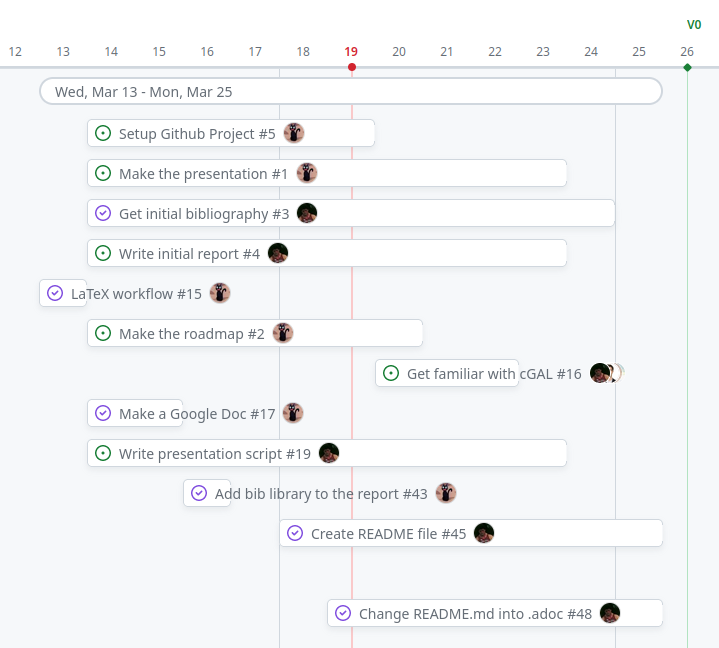
\includegraphics[width=1\textwidth]{images/roadmap_v0.png}
    \captionsetup{font={scriptsize}}
    \caption{Roadmap for V0}
\end{figure}

\begin{figure}[H]
    \centering
    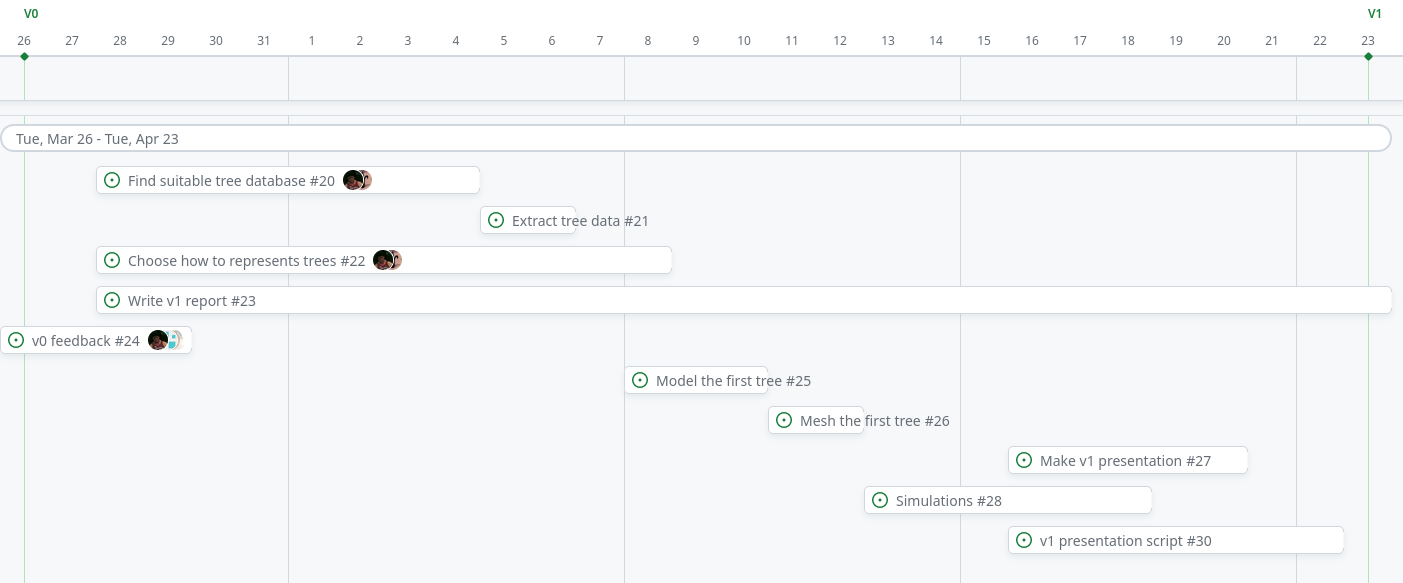
\includegraphics[width=1\textwidth]{images/roadmap_v1.png}
    \captionsetup{font={scriptsize}}
    \caption{Roadmap for V1}
\end{figure}

\begin{figure}[H]
    \centering
    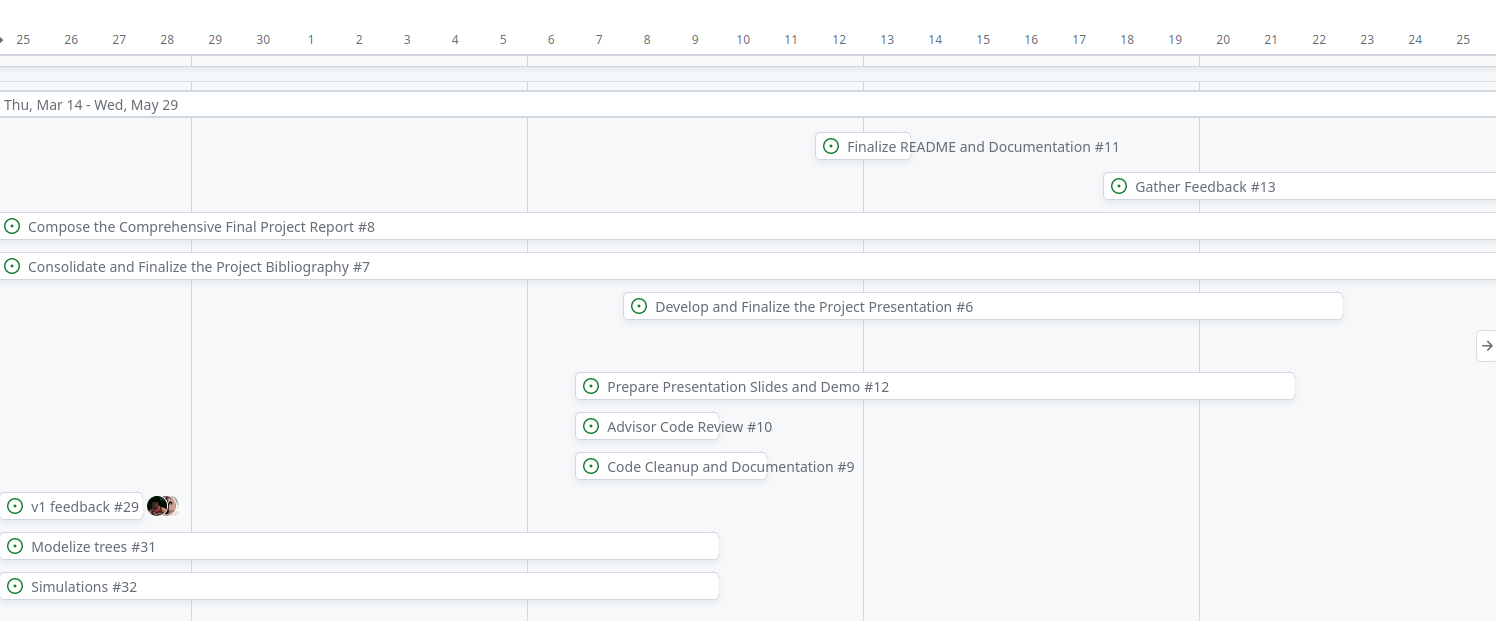
\includegraphics[width=1\textwidth]{images/roadmap_v2.png}
    \captionsetup{font={scriptsize}}
    \caption{Roadmap for V2}
\end{figure}

\newpage

\section{Introduction}
(add sources)
Urban areas are intricate environments influenced by a multitude of factors, with 
vegetation, notably trees, playing a pivotal role in shaping their microclimates 
and energy dynamics. Trees provide essential services such as shade, heat 
mitigation, and pollution reduction, making them indispensable elements in urban 
landscapes. As showed in the first image, trees can project different shadows
on the surrounding depending on the time of the day and the season making it 
more complex to model their impact on the urban environment. The second image
shows the significant impact of trees on the urban heat distribution.

\begin{figure}[H]
    \centering
    \begin{minipage}{0.45\textwidth}
        \centering
        \includegraphics[width=\textwidth]{images/TreeShade.png}
        \captionsetup{font={scriptsize}}
        \caption{Example of urban trees providing shade \cite{img:TreeShade}}
    \end{minipage}\hfill
    \begin{minipage}{0.45\textwidth}
        \centering
        \includegraphics[width=\textwidth]{images/heat_street.png}
        \captionsetup{font={scriptsize}}
        \caption{Thermal image depicting urban heat distribution \cite{img:street_thermography}}
    \end{minipage}
\end{figure}

Computational modeling has advanced significantly, enabling the simulation of thermal 
and energy performance in urban environments. However, integrating vegetation into 
these models presents challenges due to the complexity of obtaining accurate tree data 
and representing their geometry efficiently. (sources?)

\subsection{Challenges}
This project aims to address these challenges by developing a methodology for 
integrating trees into 3D urban models. Leveraging data from OpenStreetMap, the 
project will identify tree positions and attributes, generate a library of 3D tree 
models, and integrate them into terrain meshes for comprehensive simulations while
ensuring computational efficiency.

\subsection{Structure of the Report}
The following sections will be updated and completed as the project progresses.

\subsection{Data Formats and Structure}
Tree data will be sourced from OpenStreetMap and processed into formats suitable for 
integration into our models, such as .off, .csv, and .json. We aim to ensure watertight 
triangulation consistent with the Finite Element Method (FEM) for accurate simulations.  

The .off format\cite{off_format} is a simple format for 3D or 4D objects consisting of: (for 3D objects)
\begin{itemize}
    \item The keyword OFF
    \item The number of vertices, faces, and edges in order 
    \item A list of vertices: X, Y, Z coordinates
    \item A list of faces : number of vertices, vertex indices, in order (optionally, an RGB color)
\end{itemize}

\subsection{Software and Libraries}
For geometric modeling, we will utilize the CGAL \cite{cgal} library, known for its efficiency and 
reliability in geometric computation. Shading calculations will be performed using the 
Feel++ \cite{feel++} library, which specializes in solving Partial Differential Equations (PDEs) 
essential for simulating light and shade on 3D objects.

\newpage

\section{Methodology}

\subsection{Data Acquisition}
Tree data will be obtained from OpenStreetMap, providing information on tree locations, 
species, and other attributes. This data will be processed to extract relevant 
information for model integration.

\subsection{Tree Model Generation}
Using CGAL Alpha Wrapper \cite{cgal_alpha_wrapper}, 3D tree models will be generated based on the extracted data. Various 
Levels of Detail (LOD) will be considered to balance model complexity and computational 
efficiency depending on the application.

\subsection{Model Integration}
Generated tree models will be integrated into terrain meshes to create comprehensive 
3D urban models. Watertight triangulation consistent with FEM principles will be ensured 
for accurate simulations.

\subsection{Shading Calculations}
Using Feel++ ray tracing, shading effects on buildings will be simulated to account for the presence 
of trees and their impact on urban microclimates. Execution time considerations will be 
addressed to optimize computational efficiency.

\newpage

\section{Results}


\newpage

\section{Conclusion}


\newpage

\section{References}
\bibliographystyle{plain}
\bibliography{references}

\end{document}
